\section{Markets and selection}\label{sec:data}

\subsection{The two exchanges}

\paragraph{Kalshi} is a US exchange regulated by the Commodity Futures Trading Commission (CFTC). Every contract is a
yes-or-no question that pays \$1 if the answer is yes and nothing otherwise, so its price in cents reads directly as a
probability. An election appears as an \emph{event} with one market per option, for example ``Will the Democratic party
win the Senate race in Ohio?'' and the same question for the Republican party. Options are candidates in most races
and parties in some, including many of the 2024 general elections. Trading runs through an order book: traders post
bids and offers, and others take them. Kalshi charges takers a fee of 7\% of the price times one minus the price per
contract, at most 1.75 cents, and settles each market itself under written rules that name the source of the result.

\paragraph{Polymarket} is a crypto-based exchange whose contracts are tokens on a public blockchain. A winning token
pays \$1. An election appears either as a group of yes-or-no markets, one per candidate and often one for ``another
candidate'', or as a single market whose two outcomes are the two candidates. Trading also runs through an order book.
Political markets carried no trading fee until 30 March 2026; since then takers pay 4\% of the price times one minus the
price. Markets resolve through UMA's optimistic oracle: anyone can propose the outcome by posting a bond, and if nobody
challenges it within two hours the market settles; a challenged outcome goes to a vote of UMA token holders. After a
2022 settlement with the CFTC, Polymarket blocked US users for most of the period studied, and it re-entered the US
market in 2025 by buying a licensed exchange. Its prices are nonetheless among the most quoted for US elections.

\subsection{Collecting the contests}

From each exchange's public interface we downloaded every settled election market: all 2{,}062 events in Kalshi's
Elections category, and all 2{,}777 closed Polymarket events carrying any election tag. Four rules then turn events into
\emph{contests}, applied in order:
\begin{enumerate}
  \item \textbf{Two candidates.} Exactly two named options traded. An ``another candidate'' option is not a candidate,
        and placeholders that never traded are ignored.
  \item \textbf{One race.} The market pays on who wins one named race, judged by reading the titles only. Markets on
        vote shares, margins, turnout, seat counts or chamber control are dropped.
  \item \textbf{One clear winner.} Every market has settled, and exactly one option won.
  \item \textbf{One listing per race.} A race listed twice on the same exchange is kept once, the listing with more
        volume.
\end{enumerate}
Only the third rule depends on the result, and it has to. Volume is used only to tell whether an option ever traded
and to break ties between duplicate listings; prices are not used. These rules leave 391 contests on Kalshi and 224 on
Polymarket, of which 344 and 179 are in the United States. Table~\ref{tab:selection} follows the counts through every
step.

\subsection{Pricing each contest once}

Every contest is priced at a single moment: 17:00 local time in the easternmost time zone among the states voting that
day. No US state closes its polls before 18:00 local time, so this is always at least an hour before the first result
anywhere in the country. For the midterms of 3 November 2026 it is 22:00 UTC. Pricing every contest once, at the same
distance from the vote, keeps heavily traded races from dominating and keeps prices comparable across election days.

The price rules, none of which looks at the result, are:
\begin{itemize}
  \item \textbf{Kalshi.} A candidate's price is the midpoint of the best bid and offer when they are at most 10 cents
        apart; otherwise the last trade, if it was in the hour before the snapshot. Otherwise the contest is dropped.
  \item \textbf{Polymarket.} A candidate's price is Polymarket's recorded price at the snapshot. The contest is dropped
        if neither candidate traded in the day before the snapshot, or if ``another candidate'' is priced above 5\%.
  \item \textbf{Both.} A contest is dropped if any of its markets opened after the snapshot, or if the prices of all its
        options add up to less than 0.90 or more than 1.10, a sign that at least one price is stale. The two candidate
        prices are then scaled to add up to 1, and the contest is kept only if the favourite's scaled price is at most
        95\%.
\end{itemize}
The last rule removes most contests (Table~\ref{tab:rules}). A favourite above 95\% has little room to be
underpriced and carries little information about calibration, and at those prices a few cents of spread or staleness
swamp the signal. The analysis is therefore about contests with real uncertainty on election day. After all rules,
152 contests remain on Kalshi and 64 on Polymarket for the training period, November 2023 to September 2026.

\begin{table}[t]
\centering\small
\caption{Contests at each step of the selection.}\label{tab:selection}
\begin{tabular}{llrr}
\toprule
 & Step & Kalshi & Polymarket \\
\midrule
Training & Settled election events downloaded (all countries) & 2{,}062 & 2{,}777 \\
 & Two candidates, one race, one clear winner (all countries) & 391 & 224 \\
 & \quad of which in the US & 344 & 179 \\
 & Passed the price rules: \textbf{analysed} & \textbf{152} & \textbf{64} \\
\midrule
Midterms & Listed before the vote & 572 & 521 \\
 & Settled by 10 November, won by a listed candidate & 548 & 499 \\
 & Passed the price rules & 197 & 152 \\
 & Outside Georgia, Louisiana and Mississippi: \textbf{tested} & \textbf{187} & \textbf{145} \\
\bottomrule
\end{tabular}
\end{table}

\begin{table}[t]
\centering
\caption{Outcome of the price rules for US contests. Each dropped contest is counted under the first rule it
fails.}\label{tab:rules}
\small
\begin{tabular}{lrrrr}
\toprule
 & \multicolumn{2}{c}{Training} & \multicolumn{2}{c}{Midterms} \\
\cmidrule(lr){2-3}\cmidrule(lr){4-5}
 & Kalshi & Polymarket & Kalshi & Polymarket \\
\midrule
Kept & 152 & 64 & 197 & 152 \\
Favourite above 95\% & 183 & 91 & 350 & 298 \\
Neither candidate traded in the last day & -- & 8 & -- & 48 \\
``Another candidate'' above 5\% & -- & 10 & -- & 1 \\
Spread over 10 cents, no trade in the last hour & 7 & -- & 1 & -- \\
Prices add up to less than 0.90 or more than 1.10 & 1 & 5 & 0 & 0 \\
A market opened after the snapshot & 1 & 1 & 0 & 0 \\
\midrule
Total priced & 344 & 179 & 548 & 499 \\
\bottomrule
\end{tabular}
\end{table}

\subsection{The midterm contests}

The midterm sample was fixed before the vote. From every open election market in late October 2026, we listed the
contests that would be decided by the vote of 3 November, judged on titles and expiry dates only, and applied the
first, second and fourth rules above. Where a race was listed twice on the same exchange, we kept the listing whose
options were candidates rather than parties, then the one with more volume. The list, 572 contests on Kalshi and 521
on Polymarket, was archived with the rest of the pre-registration and is the universe of the test: a market created
after it was made is not part of the test. After the vote, a contest enters once it has settled with one of its two
listed candidates winning, and it is priced at 22:00 UTC on 3 November under the same rules. Contests in Georgia,
Louisiana and Mississippi were excluded in advance, because a later runoff can decide races there. By 10 November, 187
contests on Kalshi and 145 on Polymarket had settled and passed every rule; 40 more on the list had not yet settled.

\subsection{What the contests look like}

\paragraph{States.} The training contests cover 45 states and the District of Columbia, plus the nationwide
presidential race of 2024 (Figure~\ref{fig:states}). Texas, Georgia and Florida have the most, largely because of
their primaries. The midterm contests cover 36 states and are more concentrated: Texas (42) and Florida (39) together
hold almost a quarter of them. Since races in one state share voters, polls and polling errors, the intervals in
Section~\ref{sec:method} resample whole states rather than single contests.

\paragraph{Offices.} The training general elections are a mix of 2024 races: state-level presidential contests,
Senate, House and governor races (Figure~\ref{fig:offices}). The training primaries are mostly House primaries,
especially on Kalshi, which lists many low-profile districts. The midterm sample is dominated by House races (112 of 187
on Kalshi, 105 of 145 on Polymarket), with governors, senators and a long tail of other statewide offices such as
attorney general and secretary of state. Kalshi also lists state supreme court and other down-ballot races that
Polymarket does not.

\paragraph{Volume.} Primaries trade far less than general elections (Figure~\ref{fig:volume}). On Kalshi, the median
training general election traded about 330{,}000 contracts over its life and the median primary about 8{,}800, a gap of
almost forty times. On Polymarket the medians are about \$1.3 million and \$39{,}000. The midterm contests sit in
between, at a median of about 183{,}000 contracts on Kalshi and \$91{,}000 on Polymarket: there are many more of them,
and most are lower-profile races than the 2024 contests that make up most of the training general elections. Volumes
on the two exchanges are not directly comparable, because Kalshi counts contracts and Polymarket dollars.

\paragraph{How heavily favoured.} Within the 50--95\% band, primary favourites tend to be priced higher than general
election favourites, with a median scaled price of 86\% on Kalshi and 87\% on Polymarket, against 78\% and 82\% for
training general elections (Figure~\ref{fig:favourites}). The midterms fall in between, at 83\% and 84\%. A primary
favourite priced at 86\% that loses is a large surprise, which is exactly what the primaries in the training data
delivered.

\begin{figure}[p]
\centering
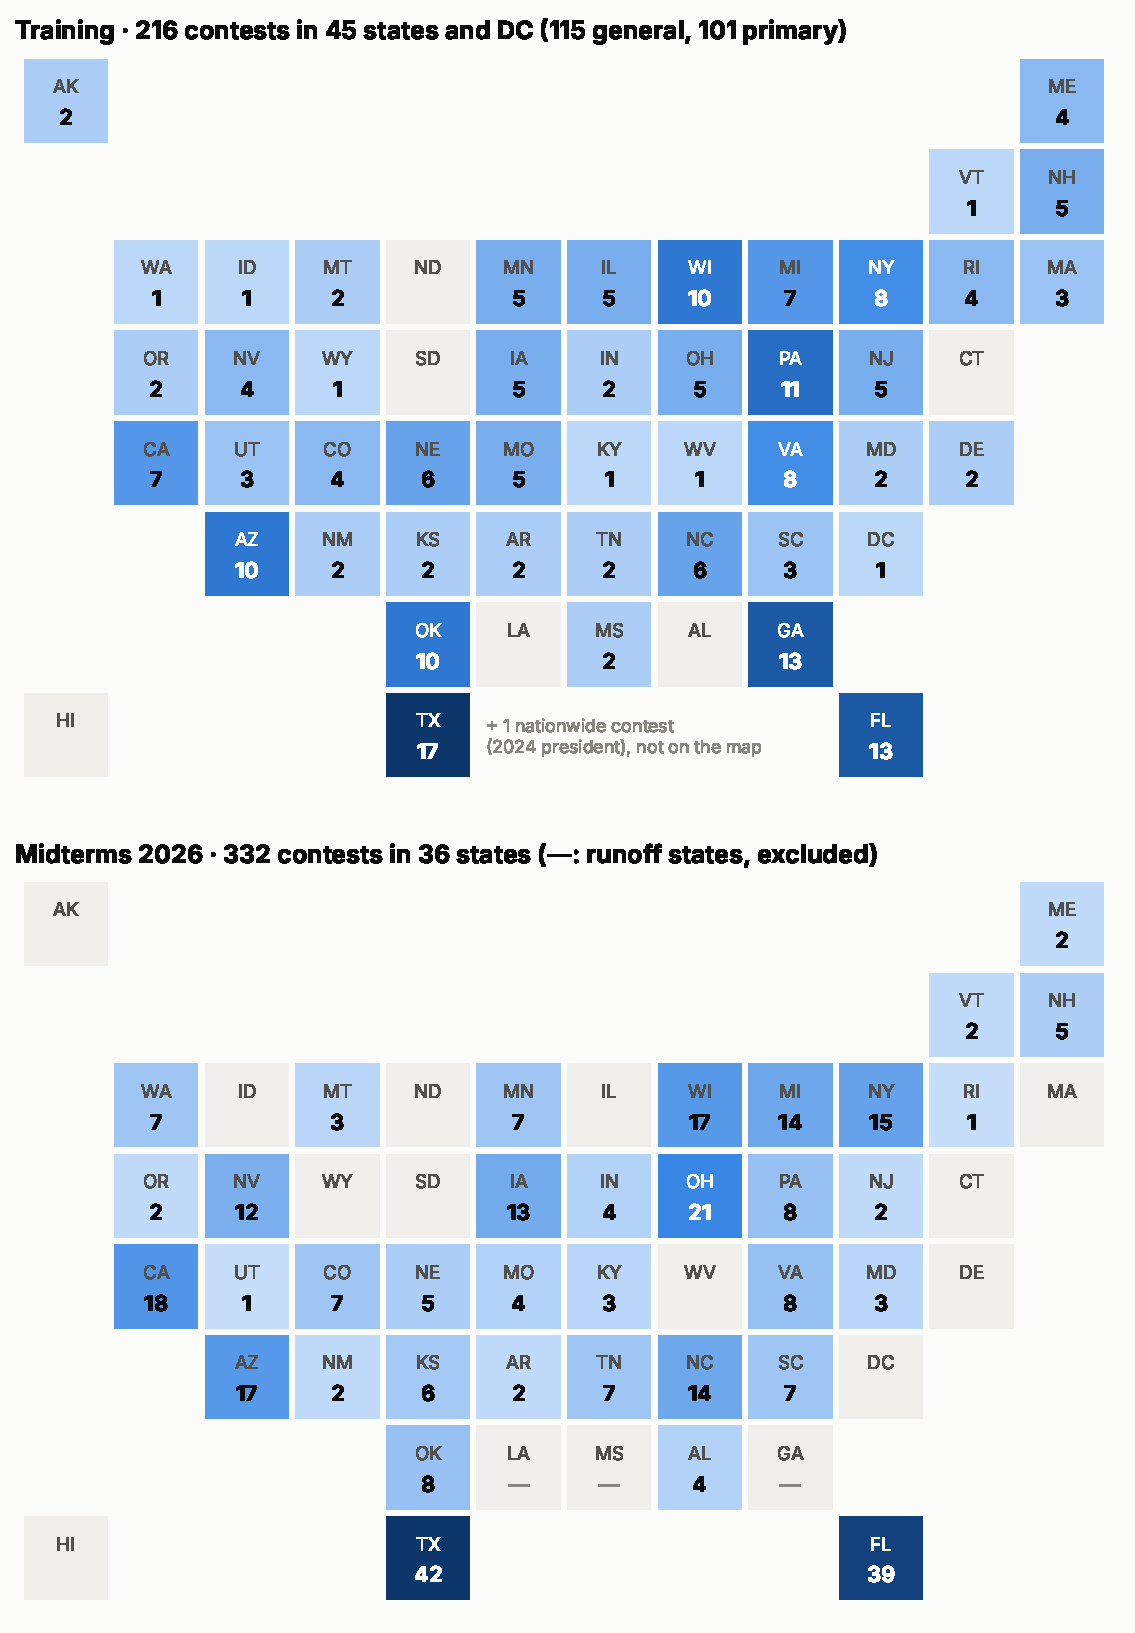
\includegraphics[width=0.78\textwidth]{figures/data_states.pdf}
\caption{Contests per state, both exchanges together. Top: the 216 training contests (general elections and
primaries). Bottom: the 332 contests in the midterm test; Georgia, Louisiana and Mississippi were excluded in advance.
Each map has its own colour scale.}\label{fig:states}
\end{figure}

\begin{figure}[t]
\centering
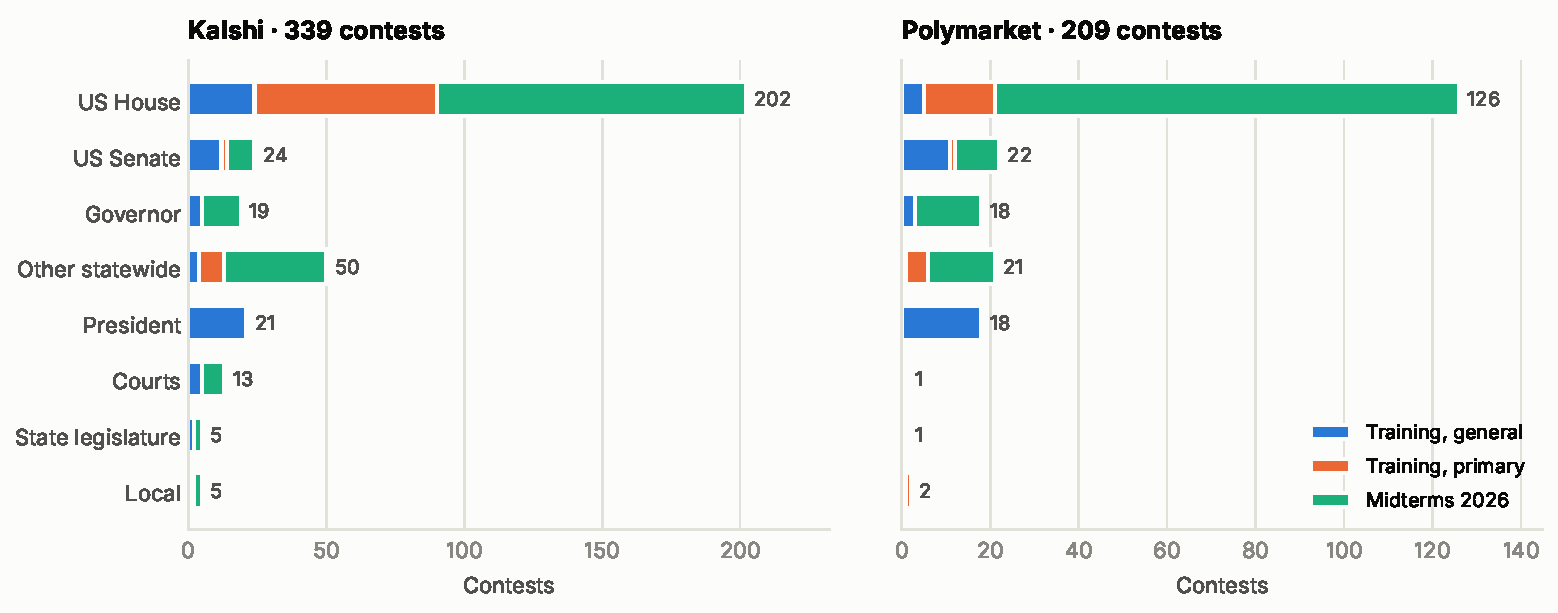
\includegraphics[width=\textwidth]{figures/data_offices.pdf}
\caption{Contests per office on each exchange, split into training general elections, training primaries and the
midterm test.}\label{fig:offices}
\end{figure}

\begin{figure}[t]
\centering
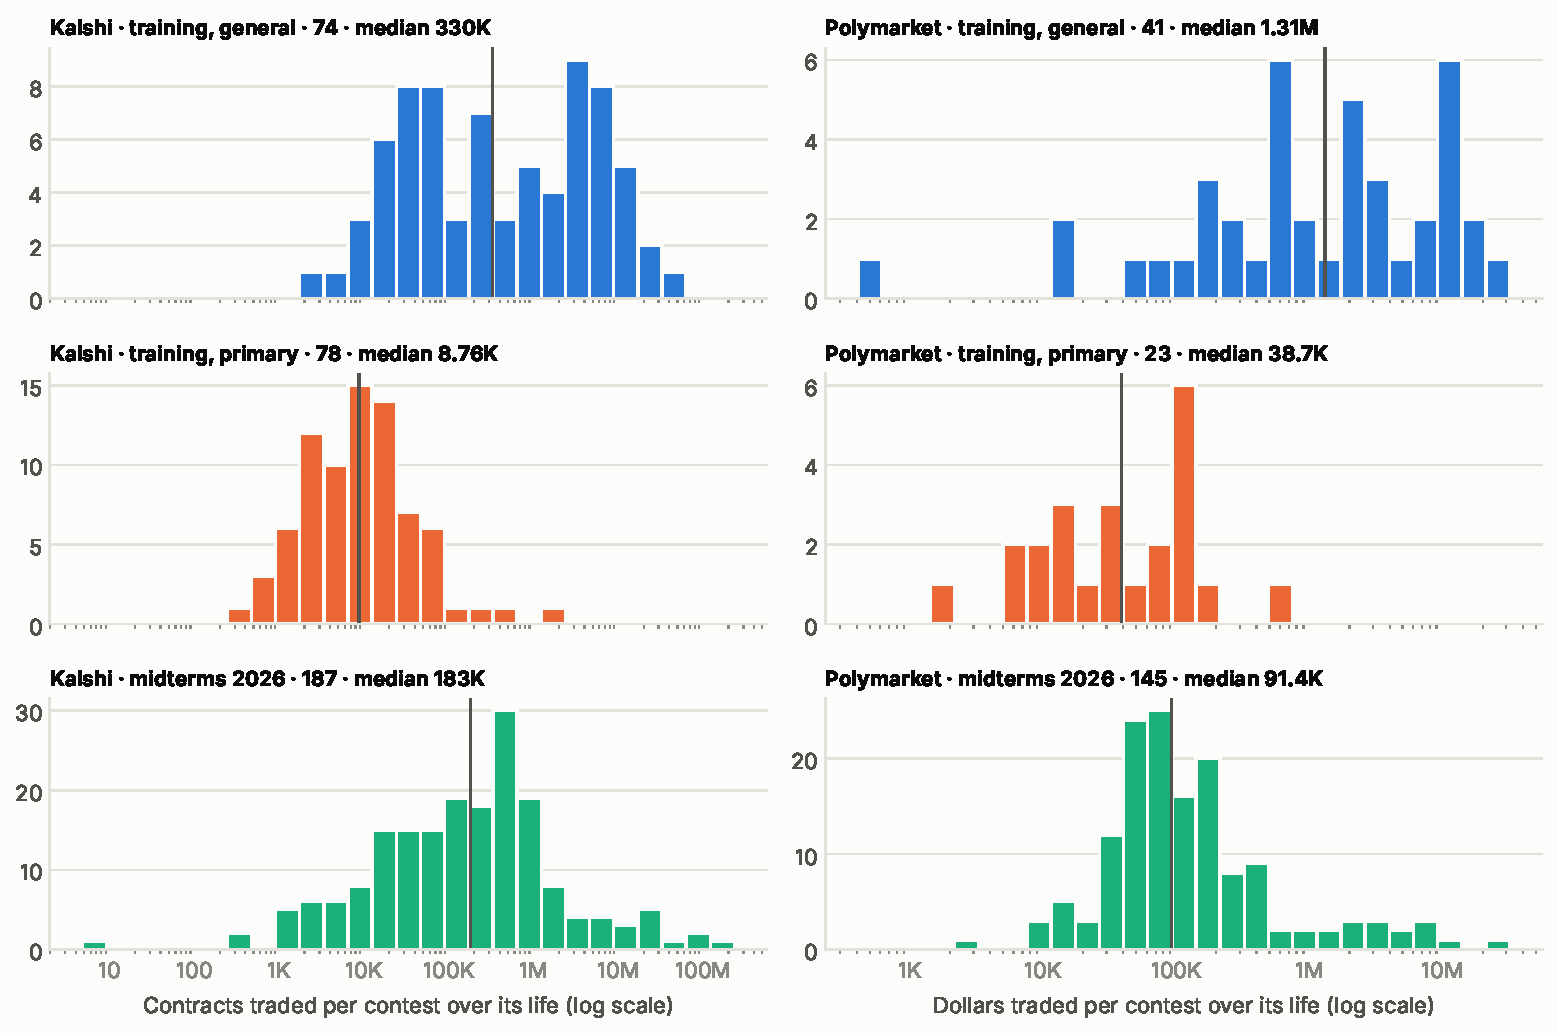
\includegraphics[width=\textwidth]{figures/data_volume.pdf}
\caption{Total volume traded per contest over its life, summed over the two candidate markets, on a log scale. The line
marks the median. Kalshi counts contracts and Polymarket dollars.}\label{fig:volume}
\end{figure}

\begin{figure}[t]
\centering
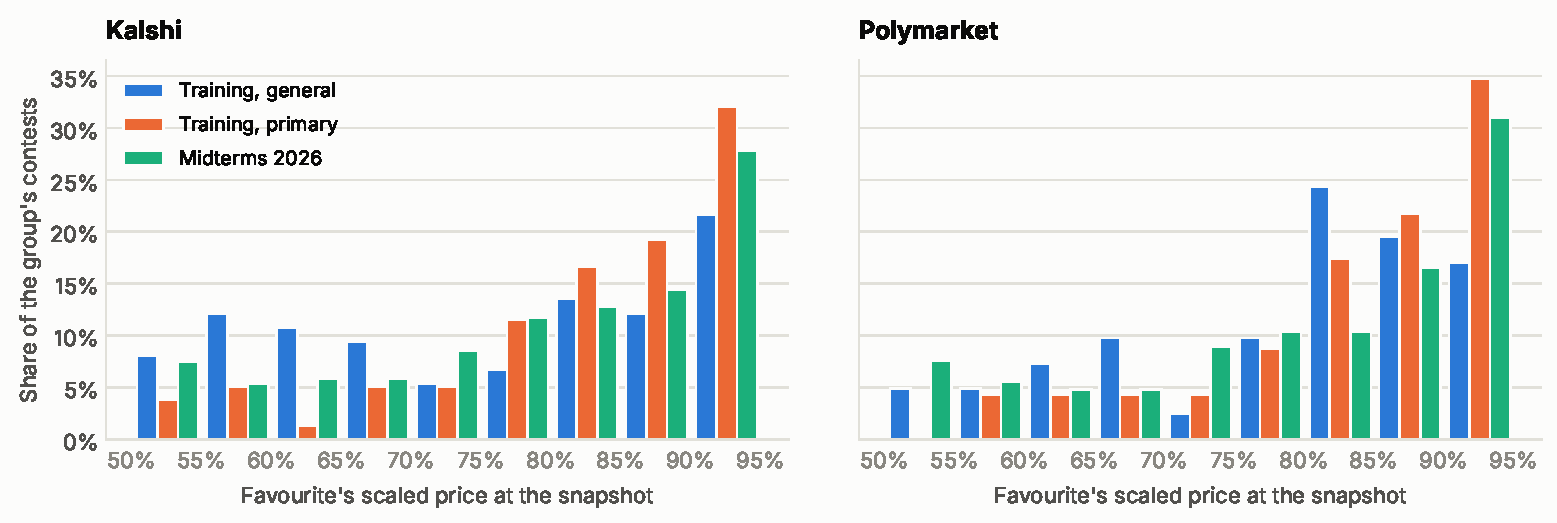
\includegraphics[width=\textwidth]{figures/data_favourites.pdf}
\caption{The favourite's scaled price at the snapshot, as a share of each group's contests. Every analysed contest lies
between 50\% and 95\% by construction.}\label{fig:favourites}
\end{figure}
